\chapter{Schroedinger equation in 2d}

Now we will turn our attention to higher dimensions, i.e 2d.
The time-independent Schrodinger equation in 2d can be written as:
\begin{equation}
\left[ -\frac{1}{2}\nabla^2 + V(x,y) \right] \psi(x,y) = E\,\psi(x,y)
\label{eq:sch_2d}
\end{equation}
%
where $\nabla^2$ is the Laplacian operator:
%
\begin{equation}
\nabla^2 = \frac{\partial^2}{\partial x^2} + \frac{\partial^2}{\partial y^2}
\end{equation}



\subsection{Describing grid in 2d}

Now we have two directions $x$ and $y$. Our approach to solving the Schroedinger equation
is similar to the one we have used before in 1d, however several technical difficulties
will arise.

To describe the computational grid, we now need to specify
$x_{\mathrm{max}}, x_{\mathrm{min}}$ for the X-domain
and $y_{\mathrm{max}}, y_{\mathrm{min}}$ for Y-domain. We also need to specify number of grid
points in for each x and y-directions, i.e. $N_{x}$ and $N_{y}$. That are quite lot of variables.
For easier management, we will collect our grid related variables in one data structure or
\txtinline{struct} in Julia. A \txtinline{struct} in Julia looks very much like C-struct.
It also defines a new custom data type in Julia.

Our struct definition looks like this.
\begin{juliacode}
struct FD2dGrid
    Npoints::Int64
    Nx::Int64
    Ny::Int64
    hx::Float64
    hy::Float64
    dA::Float64
    x::Array{Float64,1}
    y::Array{Float64,1}
    r::Array{Float64,2}
    idx_ip2xy::Array{Int64,2}
    idx_xy2ip::Array{Int64,2}
end
\end{juliacode}
%
An instance of \txtinline{FD2dGrid} can be initialized using the following constructor function:
%
\begin{juliacode}
function FD2dGrid( x_domain, Nx, y_domain, Ny )
    x, hx = init_FD1d_grid(x_domain, Nx)
    y, hy = init_FD1d_grid(y_domain, Ny)
    dA = hx*hy
    Npoints = Nx*Ny
    r = zeros(2,Npoints)
    ip = 0
    idx_ip2xy = zeros(Int64,2,Npoints)
    idx_xy2ip = zeros(Int64,Nx,Ny)
    for j in 1:Ny
        for i in 1:Nx
            ip = ip + 1
            r[1,ip] = x[i]
            r[2,ip] = y[j]
            idx_ip2xy[1,ip] = i
            idx_ip2xy[2,ip] = j
            idx_xy2ip[i,j] = ip
        end
    end
    return FD2dGrid(Npoints, Nx, Ny, hx, hy, dA, x, y, r, idx_ip2xy, idx_xy2ip) 
end
\end{juliacode}

A short explanation about the members of \txtinline{FD2dGrid} follows.
%
\begin{itemize}
%
\item \txtinline{Npoints} is the total number of grid points.
%
\item \txtinline{Nx} and \txtinline{Ny} is the total number of grid points
in $x$ and $y$-directions, respectively.
%
\item \txtinline{hx} and \txtinline{hy} is grid spacing in $x$ and $y$-directions,
respectively. \txtinline{dA} is the product of \txtinline{hx} and \txtinline{hy}.
%
\item \txtinline{x} and \txtinline{y} are the grid points in $x$ and $y$-directions.
The actual two dimensional grid points $r \equiv (x_{i},y_{i})$ are stored as
two dimensional array $r$.
%
\item Thw two integers arrays \txtinline{idx_ip2xy} and \txtinline{idx_xy2ip} defines
mapping between two dimensional grids and linear grids.
\end{itemize}


As an illustration let's build a grid for a rectangular domain
$x_\mathrm{min} = y_{\mathrm{min}}=-5$ and $x_\mathrm{max} = y_{\mathrm{max}}=5$
and $N_{x}=3$, $N_{y}=4$.
Using the above constructor for \txtinline{FD2dGrid}:
\begin{juliacode}
Nx = 3
Ny = 4
fdgrid = FD2dGrid( (-5.0,5.0), Nx, (-5.0,5.0), Ny )
\end{juliacode}
%
Dividing the $x$ and $y$ accordingly we obtain $N_{x}=3$
grid points along $x$-direction
%
\begin{textcode}
> println(fdgrid.x)
[-5.0, 0.0, 5.0]
\end{textcode}
%
and $N_{y}=4$ points along the $y$-direction
\begin{textcode}
> println(fdgrid.y)
[-5.0, -1.6666666666666665, 1.666666666666667, 5.0]
\end{textcode}
%
The actual grid points are stored in \txtinline{fdgrid.r}. Using the
following snippet, we can printout all of the grid points:
%
\begin{juliacode}
for ip = 1:fdgrid.Npoints
    @printf("%3d %8.3f %8.3f\n", ip, fdgrid.r[1,ip], fdgrid.r[2,ip])
end
\end{juliacode}
%
The results are:
%
\begin{textcode}
  1   -5.000   -5.000
  2    0.000   -5.000
  3    5.000   -5.000
  4   -5.000   -1.667
  5    0.000   -1.667
  6    5.000   -1.667
  7   -5.000    1.667
  8    0.000    1.667
  9    5.000    1.667
 10   -5.000    5.000
 11    0.000    5.000
 12    5.000    5.000
\end{textcode}
%
We also can use the usual rearrange these points in the usual 2d grid rearrangement:
%
\begin{textcode}
[  -5.000,  -5.000] [  -5.000,  -1.667] [  -5.000,   1.667] [  -5.000,   5.000] 
[   0.000,  -5.000] [   0.000,  -1.667] [   0.000,   1.667] [   0.000,   5.000] 
[   5.000,  -5.000] [   5.000,  -1.667] [   5.000,   1.667] [   5.000,   5.000]
\end{textcode}
%
which can be produced from the following snippet:
%
\begin{juliacode}
for i = 1:Nx
    for j = 1:Ny
        ip = fdgrid.idx_xy2ip[i,j]
        @printf("[%8.3f,%8.3f] ", fdgrid.r[1,ip], fdgrid.r[2,ip])
    end
    @printf("\n")
end
\end{juliacode}



\subsection{Laplacian operator}

Having built out 2d grid, we now turn our attention to the second derivative operator or
the Laplacian in the equation \ref{eq:sch_2d}.
There are several ways to build a matrix representation of the Laplacian, but we will
use the easiest one. 

Before constructing the Laplacian matrix, there is an important observation that
we should make about the second derivative matrix $\mathbb{D}^{(2)}$. We should note
that the second derivative matrix contains mostly zeros. This type of matrix that
most of its elements are zeros is called \textbf{sparse matrix}.
In a sparse matrix data structure, we only store its non-zero elements with specific
formats such as compressed sparse row/column format (CSR/CSC) and coordinate format.
We have not made use of the sparsity of the second derivative matrix
in the 1d case for simplicity. In the higher dimensions, however,
we must make use of this sparsity, otherwise we will waste computational resources 
by storing many zeros. The Laplacian matrix that we will build from
$\mathbb{D}^{(2)}$ is also very sparse.

Given second derivative matrix in $x$, $\mathbb{D}^{(2)}_{x}$,
$y$ direction, $\mathbb{D}^{(2)}_{x}$,
we can construct finite difference representation of the Laplacian operator
$\mathbb{L}$ by using
%
\begin{equation}
\mathbb{L} = \mathbb{D}^{(2)}_{x} \otimes \mathbb{I}_{y} +
\mathbb{I}_{x} \otimes \mathbb{D}^{(2)}_{y}
\end{equation}
%
where $\otimes$ is Kronecker product.
In Julia, we can use the function \jlinline{kron} to form the Kronecker product
between two matrices \jlinline{A} and \jlinline{B} as \jlinline{kron(A,B)}.

The following function illustrates the above approach to construct matrix
representation of the Laplacian operator.
\begin{juliacode}
function build_nabla2_matrix( fdgrid::FD2dGrid; func_1d=build_D2_matrix_3pt )
  Nx = fdgrid.Nx
  hx = fdgrid.hx
  Ny = fdgrid.Ny
  hy = fdgrid.hy
    
  D2x = func_1d(Nx, hx)
  D2y = func_1d(Ny, hy)

  ∇2 = kron(D2x, speye(Ny)) + kron(speye(Nx), D2y)
  return ∇2
end
\end{juliacode}

The standard Julia library does not include definition for \jlinline{speye} function
but it can be implemented by the following definition.
\begin{juliacode}
speye(N::Int64) = sparse( Matrix(1.0I, N, N) )
\end{juliacode}

In the Figure \ref{fig:fd_gaussian_2d}, an example to the approximation of 2nd derivative
of 2d Gaussian function by using finite difference is shown.

\begin{figure}[H]
{\center
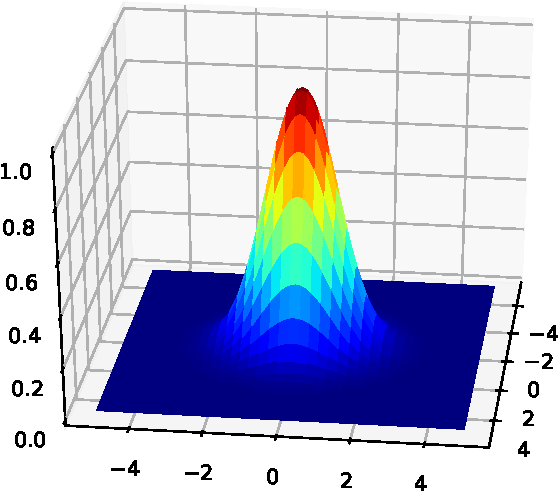
\includegraphics[width=0.45\textwidth]{../codes/FD2d/IMG_gaussian2d.pdf}\,%
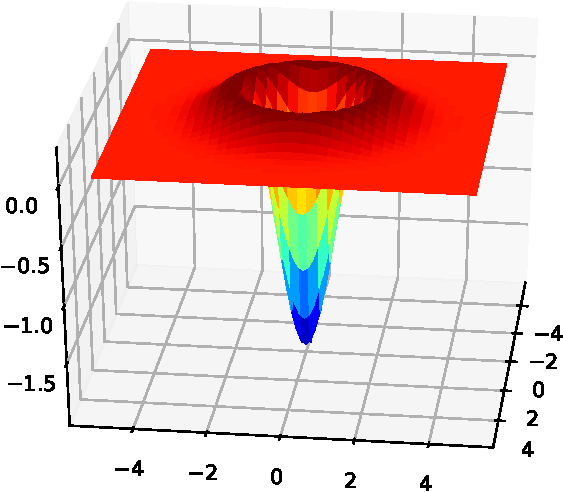
\includegraphics[width=0.45\textwidth]{../codes/FD2d/IMG_d2_gaussian2d.pdf}
\par}
\caption{Two-dimensional Gaussian function and its finite difference
approximation of second derivative}
\label{fig:fd_gaussian_2d}
\end{figure}

The following program is used to produce the figure.
\begin{juliacode}
using Printf
using LinearAlgebra
using SparseArrays
    
import PyPlot
const plt = PyPlot
    
include("FD2dGrid.jl")
include("build_nabla2_matrix.jl")
include("supporting_functions.jl")
    
function my_gaussian( fdgrid::FD2dGrid; α=1.0 )
  Npoints = fdgrid.Npoints
  f = zeros(Npoints)
  for i in 1:Npoints
    x = fdgrid.r[1,i]
    y = fdgrid.r[2,i]
    r2 = x^2 + y^2
    f[i] = exp(-α*r2)
  end
  return f
end
    
function main()  
  Nx = 75
  Ny = 75
  fdgrid = FD2dGrid( (-5.0,5.0), Nx, (-5.0,5.0), Ny )
    
  ∇2 = build_nabla2_matrix( fdgrid, func_1d=build_D2_matrix_9pt )
    
  fg = my_gaussian(fdgrid, α=0.5)
  plt.clf()
  plt.surf(fdgrid.x, fdgrid.y, reshape(fg, fdgrid.Nx, fdgrid.Ny), cmap=:jet)
  plt.gca(projection="3d").view_init(30,7)
  fileplot = "IMG_gaussian2d.pdf"
  plt.savefig(fileplot)
    
  d2fg = ∇2*fg    
  plt.clf()
  plt.surf(fdgrid.x, fdgrid.y, reshape(d2fg, fdgrid.Nx, fdgrid.Ny), cmap=:jet)
  plt.gca(projection="3d").view_init(30,7)    
  fileplot = "IMG_d2_gaussian2d.pdf"
  plt.savefig(fileplot)
end
    
main()    
\end{juliacode}


\subsection{Iterative methods for eigenvalue problem}

Now that we know how to build the Laplacian matrix, we now can build the Hamiltonian
matrix given some potential:
\begin{juliacode}
∇2 = build_nabla2_matrix( fdgrid )
Ham = -0.5*∇2 + spdiagm( 0 => Vpot )
\end{juliacode}
Note that we have used sparse diagonal matrix for building the potential matrix by
using the function \txtinline{spdiagm}.
Our next task after building the Hamiltonian matrix is to find the eigenvalues
and eigenfunctions.
However, note that the Hamiltonian matrix size is large.
For example, if we use $N_x=50$ and $N_y=50$ we will end up with a Hamiltonian
matrix with the size of $2500$.
The use of \txtinline{eigen} method, as we have done in the 1d case,
to solve this eigenvalue problem is thus not practical.
Actually, given enough computer memory and time, we can use the function
\txtinline{eigen} anyway to find all eigenvalue and eigenfunction pairs of
the Hamiltonian, however it is not recommended
nor practical for larger problem size.

Typically, we do not need to solve for all eigenvalue and eigenfunction pairs.
We only need to solve for several eigenpairs with lowest eigenvalues. In a typical density
functional theory calculations, we only need to solve for $N_{\mathrm{electrons}}$ or
$N_{\mathrm{electrons}}/2$ lowest states, where $N_{\mathrm{electrons}}$ is the number
of electrons in the system.

In numerical methods, there are several methods to search for several eigenpairs
of a matrix. These methods falls into the category of \textit{partial or iterative
diagonalization methods}. Several known methods are Lanczos method, Davidson method,
preconditioned conjugate gradients, etc.
The discussion about these methods are deferred to Appendix XXX.
We have prepared several implementation of iterative diagonalization methods
for your convenience:
\begin{itemize}
\item \txtinline{diag_Emin_PCG}
\item \txtinline{diag_davidson}
\item \txtinline{diag_LOBPCG}
\end{itemize}

These functions have similar function signatures. An example of \jlinline{diag_LOBPCG}
is given below.
\begin{juliacode}
function diag_LOBPCG!( Ham, X::Array{Float64,2}, prec;
                       tol=1e-5, NiterMax=100, verbose=false,
                       verbose_last=false, Nstates_conv=0 )
\end{juliacode}
The function accepts three mandatory arguments:
\begin{itemize}
\item \jlinline{Ham}: the Hamiltonian matrix
\item \jlinline{X::Array{Float64,2}}: initial guess of eigenfunctions
\item \jlinline{prec}: the preconditioner
\end{itemize}

Almost all iterative methods need a good preconditioner to function properly.
We will use several ready-to-use preconditioners that have been implemented
in several packages in Julia such as incomplete LU and multigrid preconditioners.

\section{2d harmonic potential}

We will test our implementation for solving Schroedinger equation for two
dimensional harmonic potentials:
\begin{equation}
V(x,y) = \frac{1}{2} \omega^2 (x^2 + y^2)
\end{equation}
This potential can be implemented in the following Julia code.
\begin{juliacode}
function pot_harmonic( fdgrid::FD2dGrid; ω=1.0 )
  Npoints = fdgrid.Npoints
  Vpot = zeros(Npoints)
  for i in 1:Npoints
    x = fdgrid.r[1,i]
    y = fdgrid.r[2,i]
    Vpot[i] = 0.5 * ω^2 *( x^2 + y^2 )
  end
  return Vpot
end
\end{juliacode}

Energy eigenvalues:
\begin{textcode}
n_x + n_y + 1  &  Values of n_x and n_y
1              &  (0,0)
2              &  (1,0) (0,1)
3              &  (2,0) (1,1) (1,1)
4              &  (3,0) (0,3) (2,1) (1,2)
\end{textcode}

Energy:
\begin{equation}
E_{n_{x} + n_{y}} = \hbar \omega \left( n_{x} + n_{y} + 1 \right)
\end{equation}

The complete program can be found in the file \txtinline{sch_2d/main_harmonic.jl}.
Here we show the main function of the program.
%
\begin{juliacode}
function main()
  Nx = 50
  Ny = 50
  fdgrid = FD2dGrid( (-5.0,5.0), Nx, (-5.0,5.0), Ny )
  ∇2 = build_nabla2_matrix( fdgrid )
  Vpot = pot_harmonic( fdgrid )
  Ham = -0.5*∇2 + spdiagm( 0 => Vpot )

  # Preconditioner based on inverse kinetic
  prec = ilu(-0.5*∇2)

  Nstates = 10
  Npoints = Nx*Ny
  X = rand(Float64, Npoints, Nstates)
  ortho_sqrt!(X)
    
  evals = diag_LOBPCG!( Ham, X, prec, verbose=true )
  X = X/sqrt(fdgrid.dA) # renormalize the eigenfunctions

  @printf("\n\nEigenvalues\n")
  for i in 1:Nstates
    @printf("%5d %18.10f\n", i, evals[i])
  end
end
\end{juliacode}

Eigenvalues ($N_{x} = N_{y} = 50$) (using 3pt):
\begin{textcode}
    Eigenvalues
    1       0.9973901176
    2       1.9921565440
    3       1.9921566198
    4       2.9816542867
    5       2.9816544298
    6       2.9869229641
    7       3.9658411776
    8       3.9658416551
    9       3.9764210096
   10       3.9764216828
\end{textcode}

Eigenvalues ($N_{x} = N_{y} = 50$) (using 9pt):
\begin{textcode}
    Eigenvalues
    1       0.9999999862
    2       1.9999998768
    3       1.9999999392
    4       2.9999992436
    5       2.9999993054
    6       2.9999997845
    7       3.9999973668
    8       3.9999976649
    9       3.9999992565
   10       3.9999998030
\end{textcode}

The eigenfunctions are shown in Figure \ref{fig:harm_2d_eigenfunctions}.

\begin{figure}[H]
{\centering
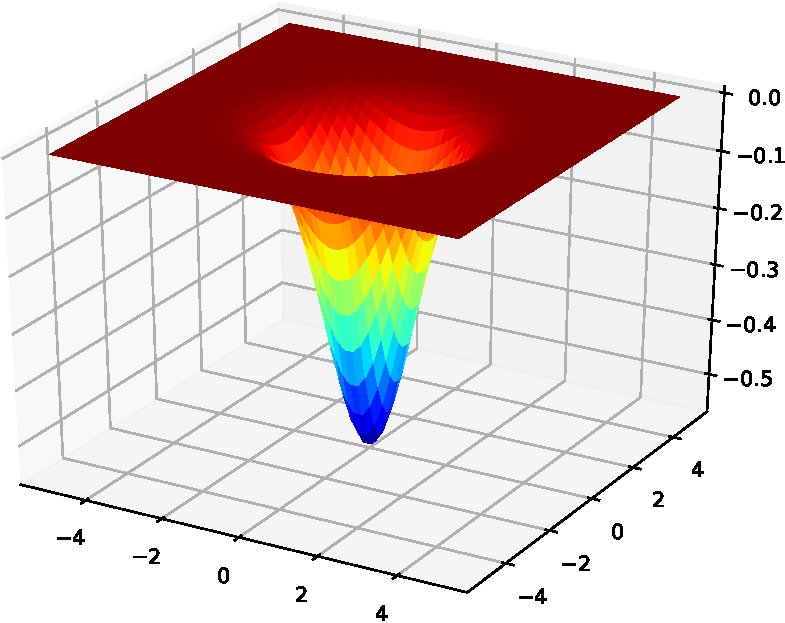
\includegraphics[scale=0.3]{../codes/sch_2d/IMG_harmonic_psi_1.pdf}\\
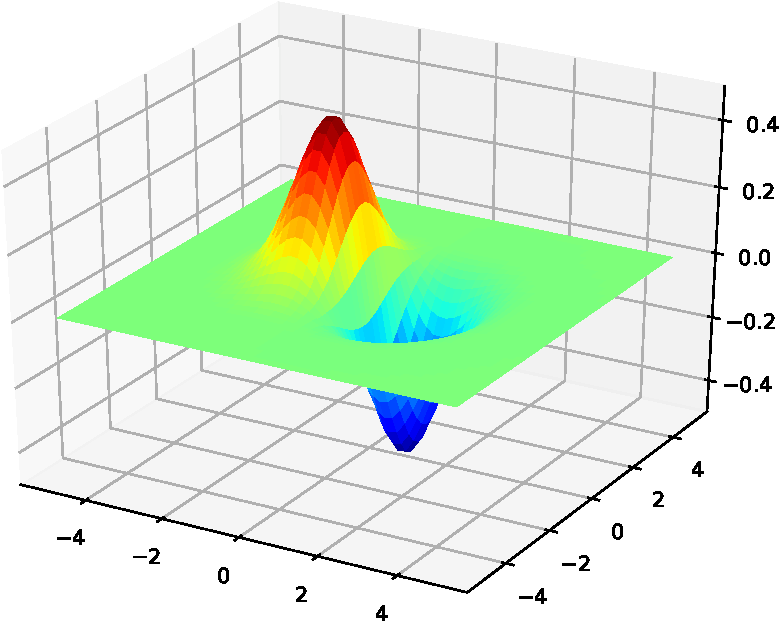
\includegraphics[scale=0.3]{../codes/sch_2d/IMG_harmonic_psi_2.pdf}%
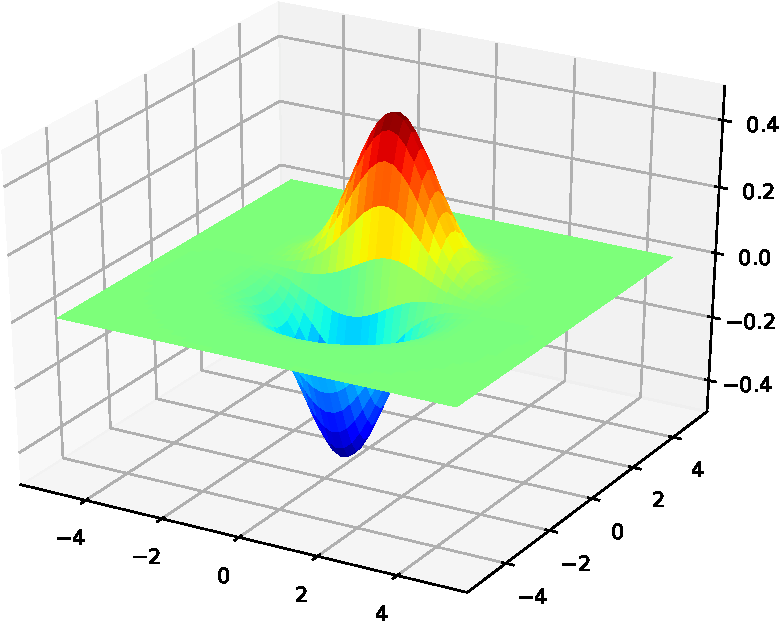
\includegraphics[scale=0.3]{../codes/sch_2d/IMG_harmonic_psi_3.pdf}\\
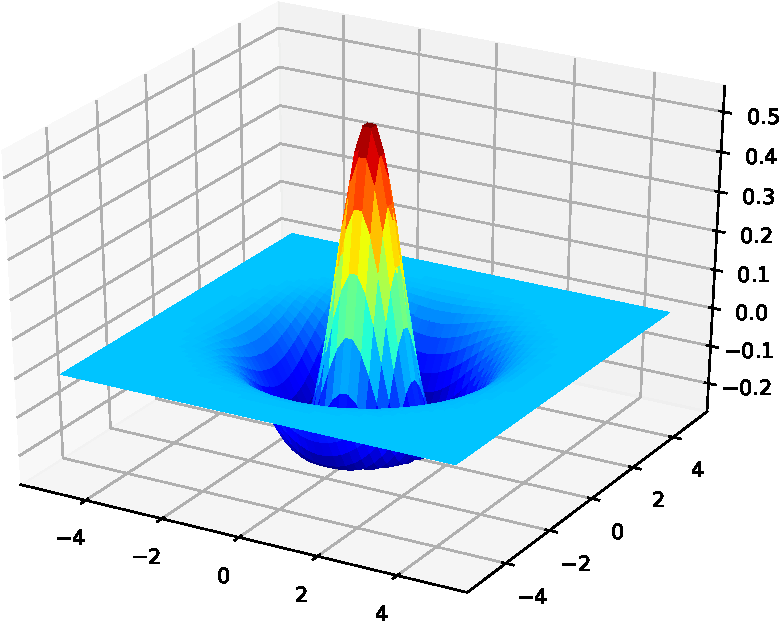
\includegraphics[scale=0.3]{../codes/sch_2d/IMG_harmonic_psi_4.pdf}%
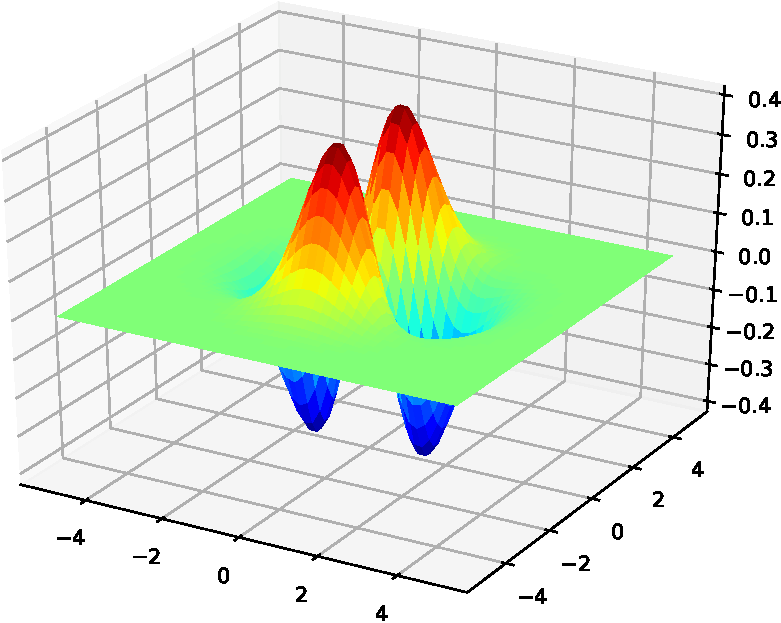
\includegraphics[scale=0.3]{../codes/sch_2d/IMG_harmonic_psi_5.pdf}%
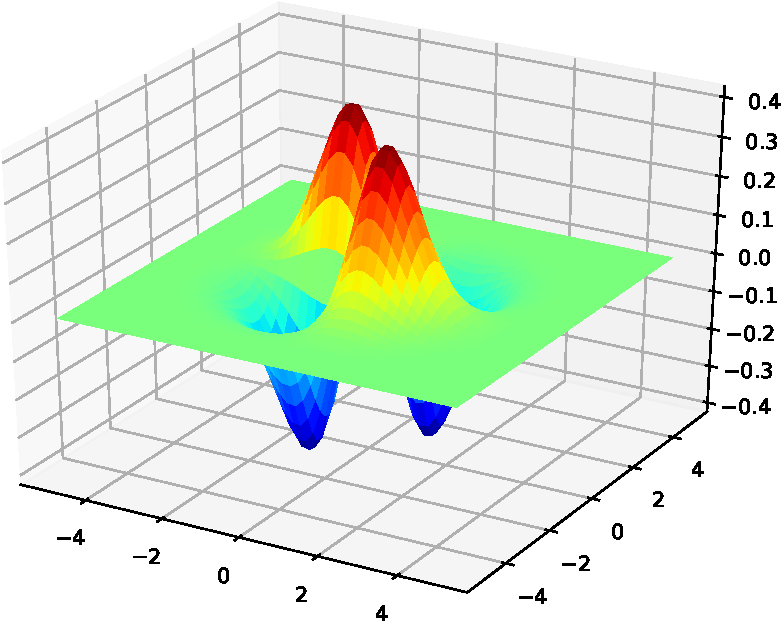
\includegraphics[scale=0.3]{../codes/sch_2d/IMG_harmonic_psi_6.pdf}\\
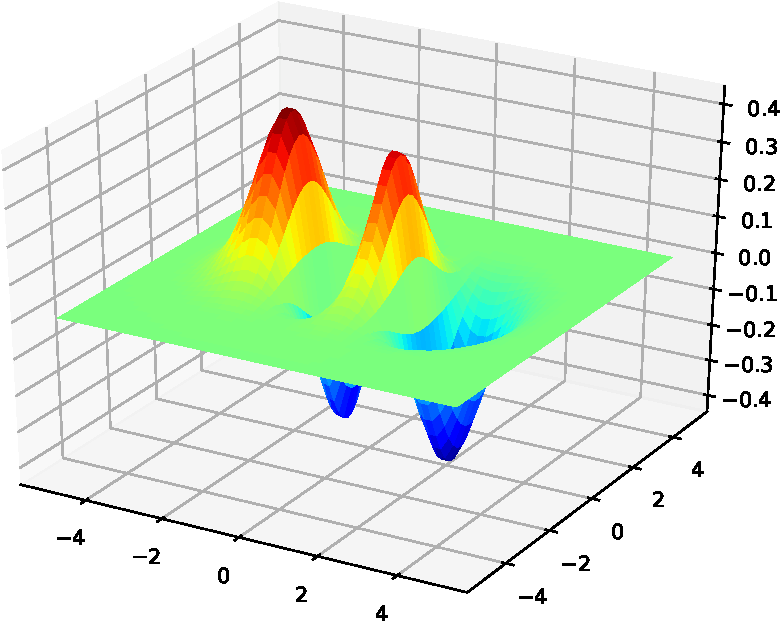
\includegraphics[scale=0.3]{../codes/sch_2d/IMG_harmonic_psi_7.pdf}%
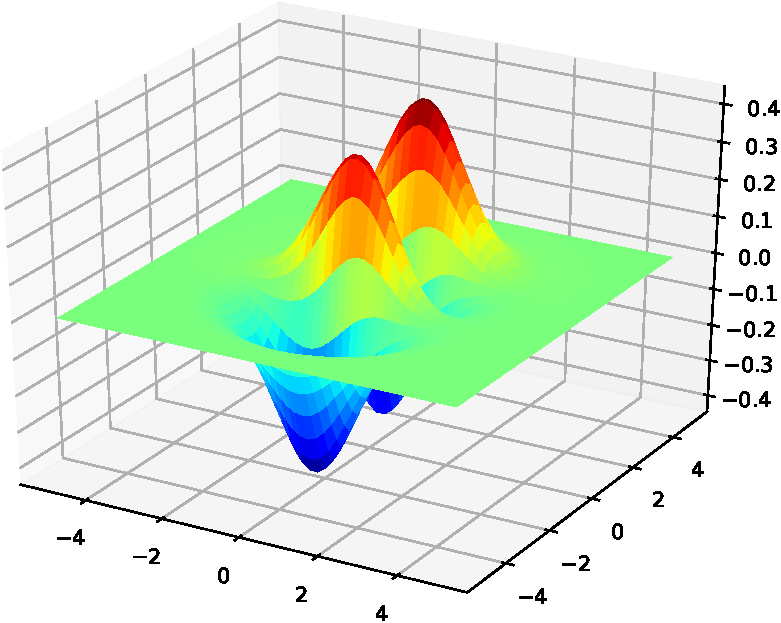
\includegraphics[scale=0.3]{../codes/sch_2d/IMG_harmonic_psi_8.pdf}%
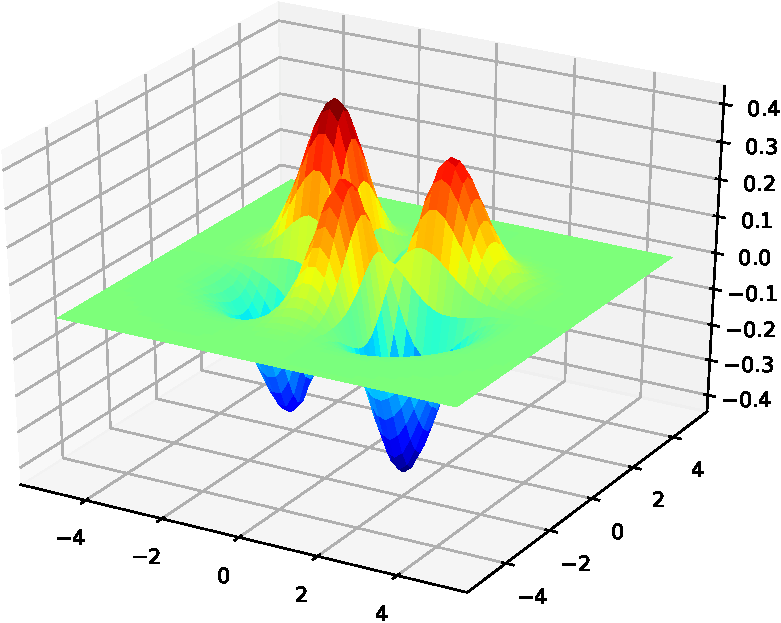
\includegraphics[scale=0.3]{../codes/sch_2d/IMG_harmonic_psi_9.pdf}%
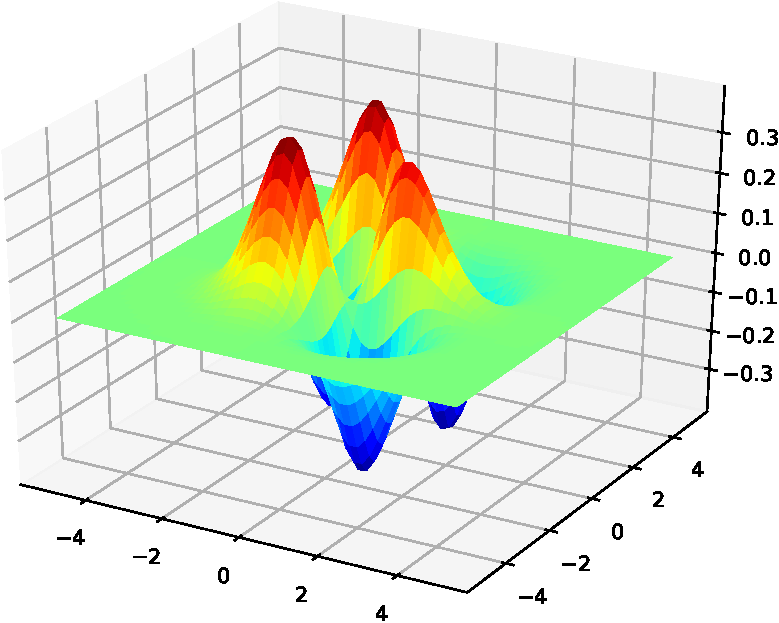
\includegraphics[scale=0.3]{../codes/sch_2d/IMG_harmonic_psi_10.pdf}
\par}
\label{fig:harm_2d_eigenfunctions}
\end{figure}

TODO: degenerate states.